\documentclass[floatsintext,man]{apa6}

\usepackage{amssymb,amsmath}
\usepackage{ifxetex,ifluatex}
\usepackage{fixltx2e} % provides \textsubscript
\ifnum 0\ifxetex 1\fi\ifluatex 1\fi=0 % if pdftex
  \usepackage[T1]{fontenc}
  \usepackage[utf8]{inputenc}
\else % if luatex or xelatex
  \ifxetex
    \usepackage{mathspec}
    \usepackage{xltxtra,xunicode}
  \else
    \usepackage{fontspec}
  \fi
  \defaultfontfeatures{Mapping=tex-text,Scale=MatchLowercase}
  \newcommand{\euro}{€}
\fi
% use upquote if available, for straight quotes in verbatim environments
\IfFileExists{upquote.sty}{\usepackage{upquote}}{}
% use microtype if available
\IfFileExists{microtype.sty}{\usepackage{microtype}}{}

% Table formatting
\usepackage{longtable, booktabs}
\usepackage{lscape}
% \usepackage[counterclockwise]{rotating}   % Landscape page setup for large tables
\usepackage{multirow}		% Table styling
\usepackage{tabularx}		% Control Column width
\usepackage[flushleft]{threeparttable}	% Allows for three part tables with a specified notes section
\usepackage{threeparttablex}            % Lets threeparttable work with longtable

% Create new environments so endfloat can handle them
% \newenvironment{ltable}
%   {\begin{landscape}\begin{center}\begin{threeparttable}}
%   {\end{threeparttable}\end{center}\end{landscape}}

\newenvironment{lltable}
  {\begin{landscape}\begin{center}\begin{ThreePartTable}}
  {\end{ThreePartTable}\end{center}\end{landscape}}




% The following enables adjusting longtable caption width to table width
% Solution found at http://golatex.de/longtable-mit-caption-so-breit-wie-die-tabelle-t15767.html
\makeatletter
\newcommand\LastLTentrywidth{1em}
\newlength\longtablewidth
\setlength{\longtablewidth}{1in}
\newcommand\getlongtablewidth{%
 \begingroup
  \ifcsname LT@\roman{LT@tables}\endcsname
  \global\longtablewidth=0pt
  \renewcommand\LT@entry[2]{\global\advance\longtablewidth by ##2\relax\gdef\LastLTentrywidth{##2}}%
  \@nameuse{LT@\roman{LT@tables}}%
  \fi
\endgroup}


  \usepackage{graphicx}
  \makeatletter
  \def\maxwidth{\ifdim\Gin@nat@width>\linewidth\linewidth\else\Gin@nat@width\fi}
  \def\maxheight{\ifdim\Gin@nat@height>\textheight\textheight\else\Gin@nat@height\fi}
  \makeatother
  % Scale images if necessary, so that they will not overflow the page
  % margins by default, and it is still possible to overwrite the defaults
  % using explicit options in \includegraphics[width, height, ...]{}
  \setkeys{Gin}{width=\maxwidth,height=\maxheight,keepaspectratio}
\ifxetex
  \usepackage[setpagesize=false, % page size defined by xetex
              unicode=false, % unicode breaks when used with xetex
              xetex]{hyperref}
\else
  \usepackage[unicode=true]{hyperref}
\fi
\hypersetup{breaklinks=true,
            pdfauthor={},
            pdftitle={TBD},
            colorlinks=true,
            citecolor=blue,
            urlcolor=blue,
            linkcolor=black,
            pdfborder={0 0 0}}
\urlstyle{same}  % don't use monospace font for urls

\setlength{\parindent}{0pt}
%\setlength{\parskip}{0pt plus 0pt minus 0pt}

\setlength{\emergencystretch}{3em}  % prevent overfull lines


% Manuscript styling
\captionsetup{font=singlespacing,justification=justified}
\usepackage{csquotes}
\usepackage{upgreek}



\usepackage{tikz} % Variable definition to generate author note

% fix for \tightlist problem in pandoc 1.14
\providecommand{\tightlist}{%
  \setlength{\itemsep}{0pt}\setlength{\parskip}{0pt}}

% Essential manuscript parts
  \title{TBD}

  \shorttitle{Entropy and Typing}


  \author{Matthew J. C. Crump\textsuperscript{1}, Walter Lai\textsuperscript{1}, \& Nicholaus Brosowsky\textsuperscript{1}}

  % \def\affdep{{"", "", ""}}%
  % \def\affcity{{"", "", ""}}%

  \affiliation{
    \vspace{0.5cm}
          \textsuperscript{1} Brooklyn College of the City University of New York  }

  \authornote{
    In this draft, listed authorship order simply indicates who is
    participating in the project
    
    Correspondence concerning this article should be addressed to Matthew J.
    C. Crump, Brooklyn College of CUNY, 2900 Bedford Avenue, Brooklyn, NY,
    11210. E-mail:
    \href{mailto:mcrump@brooklyn.cuny.edu}{\nolinkurl{mcrump@brooklyn.cuny.edu}}
  }


  \abstract{Enter abstract here. Each new line herein must be indented, like this
line.}
  \keywords{keywords \\

    \indent Word count: X
  }





\usepackage{amsthm}
\newtheorem{theorem}{Theorem}
\newtheorem{lemma}{Lemma}
\theoremstyle{definition}
\newtheorem{definition}{Definition}
\newtheorem{corollary}{Corollary}
\newtheorem{proposition}{Proposition}
\theoremstyle{definition}
\newtheorem{example}{Example}
\theoremstyle{definition}
\newtheorem{exercise}{Exercise}
\theoremstyle{remark}
\newtheorem*{remark}{Remark}
\newtheorem*{solution}{Solution}
\begin{document}

\maketitle

\setcounter{secnumdepth}{0}



Hicks Law refers to the noticeable slowing of responses in choice
reaction experiments when the possible stimuli are less predictable.

Hicks in his experiment, \enquote{On the rate of gain of information},
tested his reaction speed on a choice reaction test. During each trial
he had to determine which of n lights was turned on. He manipulated the
set size n, and found that the greater the number of alternatives the
slower his response. His data also suggested that reaction speed is
linearly related to the predictability of responses; Trials in which
certain responses were disproportionately more likely ellicited faster
response times than those in which each response was equally likely.

Hick's law at larger set sizes however does not have consistent
experimental support.

Conrad (1962) in an experiment which required subjects to name 320
nonsense syllables within trials of variable number of distinct
syllables (number of alternatives) found that the response time was
linearly correlated with the logarithm of number of alternatives.
However, Pierce and Karlin in 1957 in an experiment which required
subjects to read pages of words as quickly as possible, reported no
differences in response times between trials with set sizes that ranged
from 4 to 256 words.\\
Proctor and Schneider in a review of studies testing Hick's Law
attributes the inconsistency in large set size experiments to
differences in skill level or practice between subjects and the
arbitrariness of Stimulus Response coding/mappings when creating more
number of alternatives.

Our experiment sought to test Hick's law on typing speeds.

In this study, we used typing data from 346 typists to analyze the
effect of letter uncertainty on response times. In essence, every letter
typed represents one choice reaction test trial from Hick's experiment.
In Hick's experiment, the probability of each light turning on was
manipulated to change the H value. This is analagous to the probability
of certain letters appearing at a specific position in a word. Peter
Norvig analyzed words from numerous texts and has determined the
probability for each letter appearing at a specific position in 2 to 9
letter words.

For example, the first letter of a two letter long word is has a 9.44\%
chance to be an \enquote{a}, 14.9\% chance to be a \enquote{t}, and a
25\% chance to be an \enquote{i}. The third letter of a five letter long
word is has a 13.5\% chance as an \enquote{e}, 4.91\% chance as a
\enquote{t}, and a 11.4 \% chance as a \enquote{a}. The H indices for
each letter position - word length pair can be calculated. The H for the
1st Letter, 2-letter-long word (abbreviated 1:2) is 2.85. The H for the
3rd Letter, 5-letter-long word (abbreviated 3:5) is 3.94. The
differences in H tell us that the first letter of a two letter long word
has lower uncertainty ie. it is more predictable than the third letter
of a five letter long word.

This combination of letter probabilities creates an H value for each
unique pair of letter position and word length.

One potential problem that can hinder our experiment's ability to test
the Hick's Law is the fact that our typists vary in terms of their skill
level. This means that differences in RT between subjects will generate
noise that may hide the H effect on RTs. An advantage of testing Hick's
Law with this data set is that the stimulus response coding is
non-arbitrary. The letters that typists see on the screen correspond
exactly to the letters on their keyboards.

\section{Methods}\label{methods}

\subsection{Data analysis and
pre-processing}\label{data-analysis-and-pre-processing}

We used R (Version 3.4.2; R Core Team, 2017) and the R-packages
\emph{bindrcpp} (Version 0.2.2; Müller, 2018), \emph{Crump} (Version
1.0; Crump, 2017), \emph{data.table} (Version 1.10.4.3; Dowle \&
Srinivasan, 2017), \emph{dplyr} (Version 0.7.4; Wickham, Francois,
Henry, \& Müller, 2017), \emph{ggplot2} (Version 2.2.1; Wickham, 2009),
\emph{knitr} (Version 1.20; Xie, 2015), \emph{papaja} (Version
0.1.0.9655; Aust \& Barth, 2018), \emph{Rcpp} (Eddelbuettel, 2017;
Eddelbuettel \& Balamuta, 2017; Version 0.12.16; Eddelbuettel \&
François, 2011), \emph{RcppZiggurat} (Version 0.1.4; Eddelbuettel,
2017), and \emph{Rfast} (Version 1.8.8; Papadakis et al., 2018) for all
our analyses.

For each subject, we recorded timestamps for each keystroke using
JavaScript. We applied the following pre-processing steps. We included
IKSIs only for keystrokes involving a lower case letter, and only for
correct keystrokes that were preceded by a correct keystroke. Outlier
IKSIs were removed for each subject, on a cell-by-cell basis, using Van
Selst \& Jolicoeur's (1994) non-recursive moving criterion procedure,
which eliminated approximately X\% of IKSIs from further analysis.

\section{Results}\label{results}

\subsection{Typing Performance}\label{typing-performance}

For each subject, we calculated mean IKSIs as a function of letter
position and word length. The letter position and word length factors
were not factorially crossed. To determine whether there were
differences among the means we submitted the means to a single factor
repeated measures design with 45 levels (e.g., letter
position\textbar{}word length: 1\textbar{}1, 1\textbar{}2, 2\textbar{}2,
\ldots{} 9\textbar{}9). Figure 1 shows mean IKSIs collapsed over
subjects, as a function of letter position and word length.

\begin{figure}[htbp]
\centering
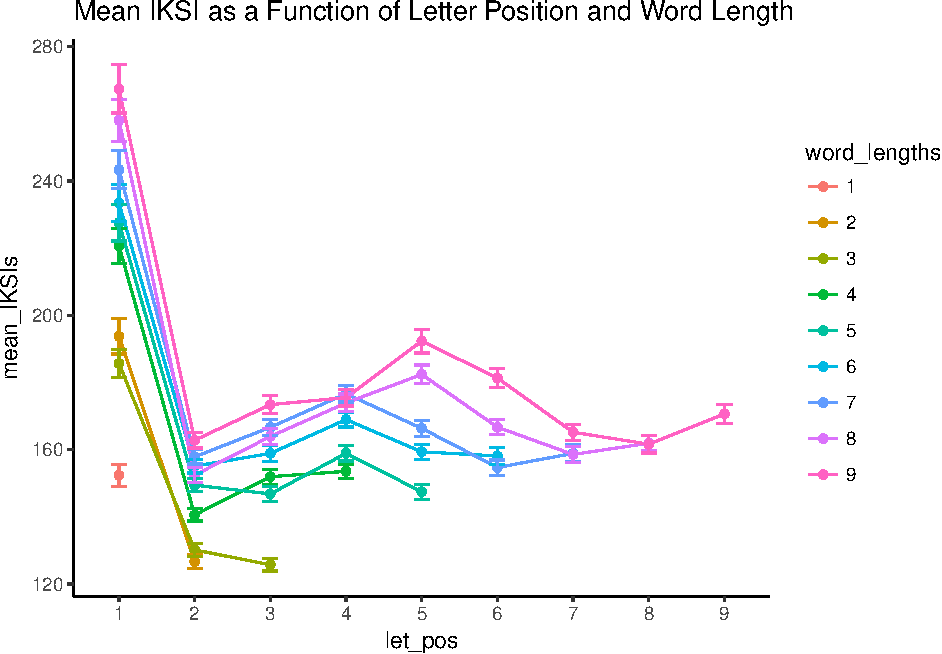
\includegraphics{Entropy_typing_draft_files/figure-latex/typing_mean_iksis_plot-1.pdf}
\caption{}
\end{figure}

The omnibus test indicated differences among the means were
significantly different from chance, F (44,15180) = 276.74, MSE =
1,269.66, p \textless{} .001. Visual inspection of figure shows several
trends across the means consistent with first-letter slowing and
mid-word slowing reported by Ostry (1983).

\begin{figure}[htbp]
\centering
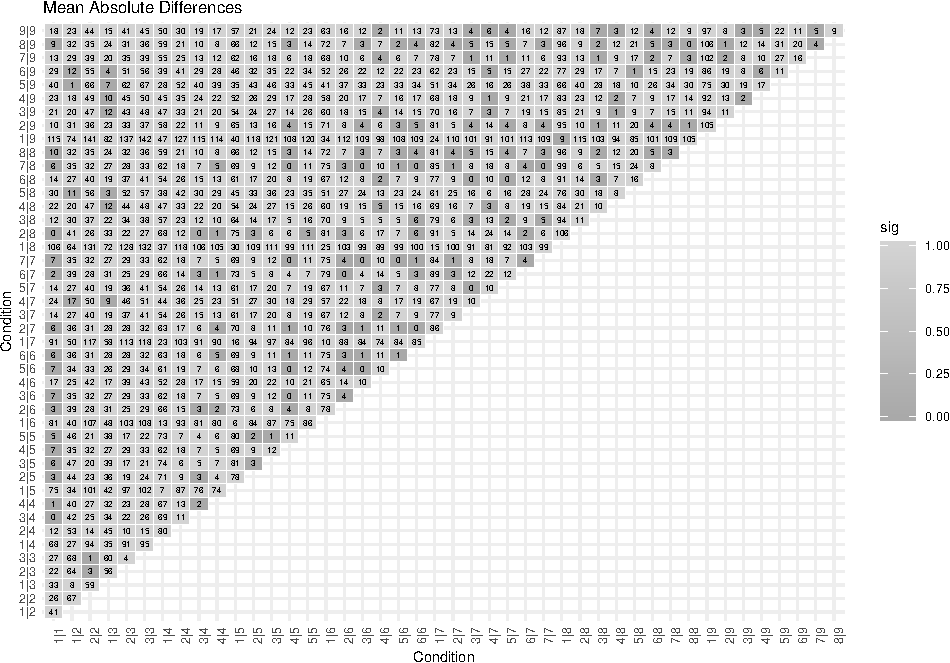
\includegraphics{Entropy_typing_draft_files/figure-latex/typing_mean_iksis_comparisons-1.pdf}
\caption{}
\end{figure}

Our more important aim was to determine whether variation among these
means can be explained by variation in letter uncertainty. For this
reason we do not exhaustively discuss all of the possible 990
differences among these 45 conditions. Nevertheless, we did conduct all
990 comparisons using bonferroni corrected paired samples t-tests. The
results are displayed Figure 2, which shows absolute mean differences
between conditions color coded for significance (light grey is
significant).

\subsection{Letter Uncertainty}\label{letter-uncertainty}

The primary question of interest was whether natural variation in letter
uncertainty by position and word length explains variance in mean IKSI
by position and word length. We estimated letter uncertainty by position
and word length from google's ngram database, which provides frequency
counts of letters and words occuring in Google's massive corpus (X
million) of digitized books. Letter frequency counts for letters a to z,
for each position in words from length one to nine, were obtained from
Norvig ().

For each letter frequency distribution, we computed Shannon's H
(entropy) to quantify letter uncertainty. Shannon's H is defined as:

\(H = -\sum p \log_2 p\)

where, p is the probability of occurence for each letter in a given
distribution. H is the number of bits needed to represent the
distribution. We considered only the set of the 26 lowercase letters
from a to z. For this set, H can range from 0 to \textasciitilde{}4.7. H
approaches 4.7 as letter probabilities approach a uniform distribution,
indicating all letters are equiprobable,
\(H = -\sum \frac{1}{26} \log_2 \frac{1}{26} = 4.7004\). H by definition
less than 4.7 for all unequal letter probability distributions, where
some letters occur with higher/lower probabilities than others.

We converted each letter frequency distribution to a probability
distribution then calculated H for each distribution. Figure 3 displays
estimates of letter uncertainty (H) as a function of letter position and
word length. Visual inspection of the graph shows that variation in
letter uncertainty maps closely onto variation in mean IKSI (Figure 1)
as a function of position and word length. In particular, letter
uncertainty and mean IKSI for position one as a function of word length
appear highly similar. And for the remaining positions, letter
uncertainty shows an inverted U- shape with greater letter uncertainty
in the middle rather than the beginning and endings of words. This
suggests that natural variation of letter uncertainty across position
and word in English may account for aspects of the first-letter and
mid-word slowing phenomena in typing.

\begin{figure}[htbp]
\centering
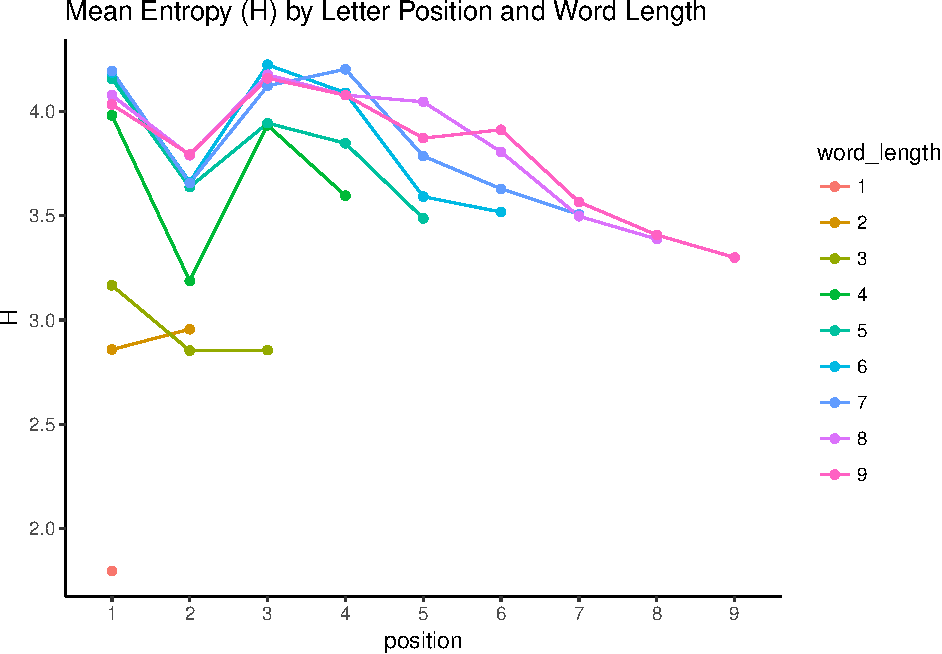
\includegraphics{Entropy_typing_draft_files/figure-latex/letter_uncertainty-1.pdf}
\caption{}
\end{figure}

\section{Letter Uncertainty and Mean
IKSI}\label{letter-uncertainty-and-mean-iksi}

If the Hick-Hyman law applied to continuous typing we would expect a
neat linear relationship between mean IKSIs and letter uncertainty.
Figure 4 shows a plot of mean IKSIs taken from all positions and word
lengths against letter uncertainty. The scatterplot shows a general
trend for mean IKSI to increase as a function of letter uncertainty.

\begin{figure}[htbp]
\centering
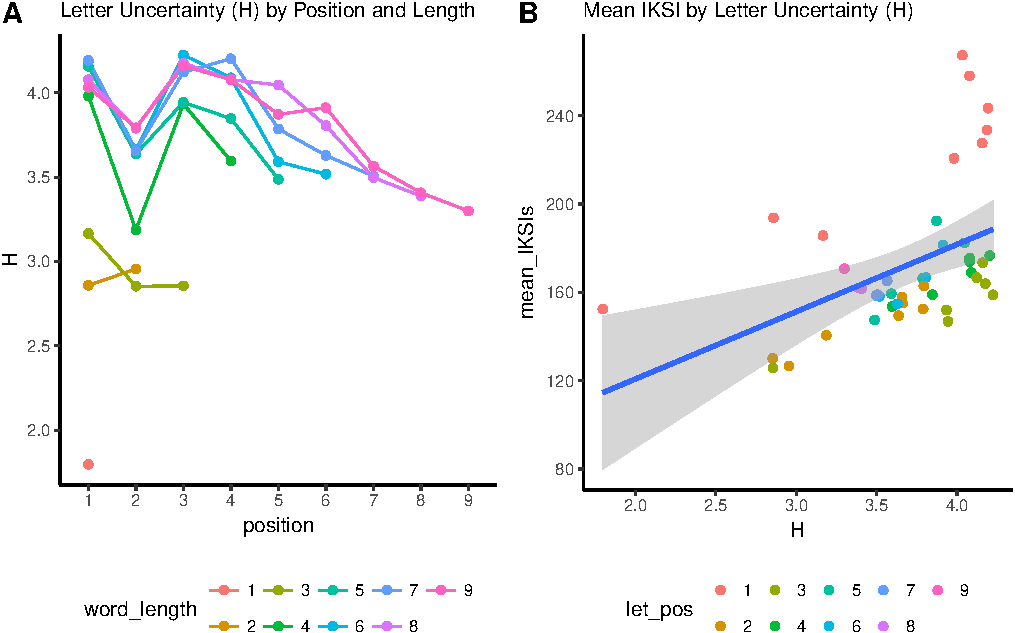
\includegraphics{Entropy_typing_draft_files/figure-latex/letter_uncertainty_by_IKSI-1.pdf}
\caption{}
\end{figure}

A linear regression on the mean IKSIs collapsed over subjects as the
dependent variable, and letter uncertainty as the independent variable
showed a significant positive correlation, r = 0.46, r\^{}2 = 0.22 , p =
0.0013

\section{Discussion}\label{discussion}

The takeaway from this experiment was that a typist types a letter
faster when the letters commonly found at the given letter position are
few. These findings are consistent with Hick's Law. As the alternatives
become equiprobable, as it is observed in the middle of words, the
number of bits required to process the choices increases.

\section{Conclusion}\label{conclusion}

Future studies should investigate the role of probability of repetition
in regulating response times.\\
Kornblum in 1969 found that with constant H, trials that had higher
chances of sequentially repeating stimuli experienced faster response
times.

\newpage

\section{References}\label{references}

\begingroup
\setlength{\parindent}{-0.5in} \setlength{\leftskip}{0.5in}

\hypertarget{refs}{}
\hypertarget{ref-R-papaja}{}
Aust, F., \& Barth, M. (2018). \emph{papaja: Create APA manuscripts with
R Markdown}. Retrieved from \url{https://github.com/crsh/papaja}

\hypertarget{ref-R-Crump}{}
Crump, M. (2017). \emph{Crump: Crump lab functions}.

\hypertarget{ref-R-data.table}{}
Dowle, M., \& Srinivasan, A. (2017). \emph{Data.table: Extension of
`data.frame`}. Retrieved from
\url{https://CRAN.R-project.org/package=data.table}

\hypertarget{ref-R-RcppZiggurat}{}
Eddelbuettel, D. (2017). \emph{RcppZiggurat: 'Rcpp' integration of
different ``ziggurat'' normal rng implementations}. Retrieved from
\url{https://CRAN.R-project.org/package=RcppZiggurat}

\hypertarget{ref-R-Rcpp_b}{}
Eddelbuettel, D., \& Balamuta, J. J. (2017). Extending extitR with
extitC++: A Brief Introduction to extitRcpp. \emph{PeerJ Preprints},
\emph{5}, e3188v1.
doi:\href{https://doi.org/10.7287/peerj.preprints.3188v1}{10.7287/peerj.preprints.3188v1}

\hypertarget{ref-R-Rcpp_a}{}
Eddelbuettel, D., \& François, R. (2011). Rcpp: Seamless R and C++
integration. \emph{Journal of Statistical Software}, \emph{40}(8),
1--18.
doi:\href{https://doi.org/10.18637/jss.v040.i08}{10.18637/jss.v040.i08}

\hypertarget{ref-R-bindrcpp}{}
Müller, K. (2018). \emph{Bindrcpp: An 'rcpp' interface to active
bindings}. Retrieved from
\url{https://CRAN.R-project.org/package=bindrcpp}

\hypertarget{ref-R-Rfast}{}
Papadakis, M., Tsagris, M., Dimitriadis, M., Fafalios, S., Tsamardinos,
I., Fasiolo, M., \ldots{} Lakiotaki, K. (2018). \emph{Rfast: A
collection of efficient and extremely fast r functions}. Retrieved from
\url{https://CRAN.R-project.org/package=Rfast}

\hypertarget{ref-R-base}{}
R Core Team. (2017). \emph{R: A language and environment for statistical
computing}. Vienna, Austria: R Foundation for Statistical Computing.
Retrieved from \url{https://www.R-project.org/}

\hypertarget{ref-R-ggplot2}{}
Wickham, H. (2009). \emph{Ggplot2: Elegant graphics for data analysis}.
Springer-Verlag New York. Retrieved from \url{http://ggplot2.org}

\hypertarget{ref-R-dplyr}{}
Wickham, H., Francois, R., Henry, L., \& Müller, K. (2017). \emph{Dplyr:
A grammar of data manipulation}. Retrieved from
\url{https://CRAN.R-project.org/package=dplyr}

\hypertarget{ref-R-knitr}{}
Xie, Y. (2015). \emph{Dynamic documents with R and knitr} (2nd ed.).
Boca Raton, Florida: Chapman; Hall/CRC. Retrieved from
\url{https://yihui.name/knitr/}

\endgroup






\end{document}
